\section{Chemins optimaux}

\frame{
    \frametitle{Définitons}

    \definition[graphe valué]{%
        Un graphe valué est un triplet $\grapheval{}$ où $(\sommets{}, \arcs{})$ est un graphe et $\cout{}: \arcs{}\rightarrow \mathbb{R}$ est une fonction de coût.
    }

    \definition[coût d'un chemin]{%
        Soit $\grapheval{}$ un graphe valué, soit $\chemin{} = \sommet{}_1,\dots,\sommet{}_n$ un chemin de $(\sommets{}, \arcs{})$, le coût de $\chemin{}$ est 
        $$\cout{}(\chemin{}) = \sum_{i=2}^{n}\cout{}((\sommet{}_{i-1}, \sommet{}_i))$$
    }

    \definition[chemin de coût minimal]{%
        Soit $\grapheval{}$ un graphe valué.
        Un chemin $\chemin{}$ de $\sommet{}$ à $\sommetb{}$ est un chemin de coût minimal si $\forall \chemin{}'$ chemin de $\sommet{}$ à $\sommetb{}$ on a $\cout{}(\chemin{}') \geq \cout{}(\chemin{})$.
    }
}

\frame{
    \frametitle{Les problèmes qu'on se pose}

    \definition[\pbvv{}]{%
        Trouver un chemin de coût minimal de $\sommet{}$ à $\sommetb{}$.
    }

    \definition[\pbvetoile{}]{%
        Pour tout $\sommetb{}$, trouver un chemin de coût minimal de $\sommet{}$ à $\sommetb{}$.
    }

    \definition[\pbetoileetoile{}]{%
        Pour tout $\sommet{}$ et tout $\sommetb{}$, trouver un chemin de coût minimal de $\sommet{}$ à $\sommetb{}$.
    }   
}

\frame{
    \frametitle{Les problèmes qu'on se pose, suite}

    \exercice{%
        \begin{center}
            \begin{tikzpicture}
                \node (v3) at (0,0) {$\sommet{}_3$};
                \node (v4) at (3,0) {$\sommet{}_4$};
                \node (v1) at (0,3) {$\sommet{}_1$};
                \node (v2) at (3,3) {$\sommet{}_2$};
                \node (v5) at (6,0) {$\sommet{}_5$};

                \shiftdraw{v1}{v2}{0}{0};
                \shiftdraw{v1}{v4}{0}{0};
                \shiftdraw{v2}{v4}{0}{0};
                \shiftdraw{v3}{v1}{0}{0};
                \shiftdraw{v4}{v3}{0}{0};
                \shiftdraw{v5}{v4}{0}{0}; 

                \node (info) at (1.5, 3.2) {2};
                \node (info) at (1.5, -0.2) {2};
                \node (info) at (-0.2, 1.5) {2};
                \node (info) at (3.2, 1.5) {2};
                \node (info) at (4.5, -0.2) {0};
                \node (info) at (1.7, 1.7) {-1};
            \end{tikzpicture}
        \end{center}

        \begin{itemize}
            \item Résoudre \pbvv{} pour $\sommet{}=\sommet{}_1$ et $\sommetb{}=\sommet{}_3$.
            \item Résoudre \pbvetoile{} pour $\sommet{}=\sommet{}_1$.
            \item Résoudre \pbetoileetoile{}.
        \end{itemize}
    }
}

\subsection{Depuis un sommet}

\frame{
    \frametitle{Circuits et chemins de coût minimal}

    \definition[circuit]{
        Soit $\graphedef{}$ un graphe. Un chemin de $\sommet{}$ à $\sommetb{}$ dans $\graphe{}$ est appelé circuit si $\sommet{} = \sommetb{}$.
    }

    \definition[circuit absorbant]{
        Un circuit $\chemin{}$ d'un graphe valué $\grapheval{}$ est dit absorbant si $\cout{}(\chemin{}) < 0$.
    }

    \pause

    \proposition{%
        Soit $\sommet{}$ un sommet d'un graphe (valué) $\graphe{}$.
        Le problème \pbvetoile{} admet une solution si et seulement si il n'existe pas de circuit absorbant atteignable depuis $\sommet{}$ dans $\graphe{}$.
    }
}

\frame{
    \frametitle{Preuve de la proposition}

    \proposition[lemme]{%
        Si un graphe $\graphe{}$ n'a pas de circuit absorbant alors pour tout chemin $\chemin{}$ de $\sommet{}$ à $\sommetb{}$ de $\graphe{}$ il existe un chemin $\chemin{}'$ extrait de $\chemin{}$ tel que~:
        \begin{itemize}
            \item $\chemin{}'$ est élémentaire,
            \item $\cout{}(\chemin{}') \leq \cout{}(\chemin{})$.
        \end{itemize}
    }

    \proposition[lemme]{%
        Dans tout graphe $\graphe{}$ il existe un nombre fini de chemins élémentaires.
    }

    \exercice[preuve de la proposition précédente]{%
        \begin{itemize}
            \item Prouver les deux lemmes.
            \item En déduire que si un graphe n'a pas de circuit absorbant alors \pbvetoile{} admet une solution.
            \item Montrer (par la contraposée) que si \pbvetoile{} admet une solution alors le graphe n'a pas de circuit absorbant.
        \end{itemize}
    }
}

\subsection{Algorithme de Bellman-Ford}

\frame{
    \frametitle{Présentation de l'algorithme de Bellman-Ford}

    L'algorithme de Bellamn-Ford calcule les chemins de coût minimal d'une source aux autres sommets dans un graphe valué, c'est-à-dire qu'il \enavant{résout \pbvetoile{}}.
    De plus, il \enavant{détecte les circuits absorbants}.
    
    \begin{center}
        \begin{minipage}{9cm}
            \begin{algorithmic}
                \In{$\grapheval{}$, $\sommet{}_0\in\sommets{}$}
                \Out{d, pred, vrai/faux}
                \State $d(\sommet{}_0) = 0, \forall \sommet{}\in\sommets{}, \sommet{}\neq\sommet{}_0, d(\sommet{}) = +\infty$
                \For{$\taille{\sommets{}} - 1$ fois}
                    \ForAll{$(\sommet{}, \sommetb{})\in \arcs{}$}
                        \If{$d(\sommetb{}) > d(\sommet{}) + \cout{}((\sommet{}, \sommetb{}))$}
                            \State $d(\sommetb{}) = d(\sommet{}) + \cout{}((\sommet{}, \sommetb{}))$ \enavant{// relachement}
                            \State $pred(\sommetb{}) = \sommet{}$
                        \EndIf
                    \EndFor
                \EndFor
                \ForAll{$(\sommet{}, \sommetb{})\in \arcs{}$}
                    \If{$d(\sommetb{}) > d(\sommet{}) + \cout{}((\sommet{}, \sommetb{}))$}
                        \State {\bf return} faux
                    \EndIf
                \EndFor
                \State {\bf return} vrai
            \end{algorithmic}
        \end{minipage}
    \end{center}
}

\frame{
    \frametitle{Exemple}

    \exercice{%
        Appliquer l'alogrithme de Bellman-Ford au graphe suivant pour $\sommet{}_0 = \sommet{}_1$.
        \begin{center}
            \begin{tikzpicture}
                \node (v3) at (0,0) {$\sommet{}_3$};
                \node (v4) at (3,0) {$\sommet{}_4$};
                \node (v1) at (0,3) {$\sommet{}_1$};
                \node (v2) at (3,3) {$\sommet{}_2$};
                \node (v5) at (6,0) {$\sommet{}_5$};

                \shiftdraw{v1}{v2}{0}{0};
                \shiftdraw{v1}{v4}{0}{0};
                \shiftdraw{v2}{v4}{0}{0};
                \shiftdraw{v3}{v1}{0}{0};
                \shiftdraw{v4}{v3}{0}{0};
                \shiftdraw{v5}{v4}{0}{0}; 

                \node (info) at (1.5, 3.2) {2};
                \node (info) at (1.5, -0.2) {2};
                \node (info) at (-0.2, 1.5) {2};
                \node (info) at (3.2, 1.5) {2};
                \node (info) at (4.5, -0.2) {0};
                \node (info) at (1.7, 1.7) {-1};
            \end{tikzpicture}
        \end{center}
    }
}

\frame{
    \frametitle{Coût d'un chemin de coût minimal}

    \notation{%
        Dans un graphe $\graphe{}$, pour tout $\sommet{}$ et tout $\sommetb{}$, on note $\coutmin{\sommet{}}{\sommetb{}}$ le coût d'un chemin de coût minimal de $\sommet{}$ à $\sommetb{}$.
    }

    \remarque{%
        Ce coût peut être $+\infty$ s'il n'existe pas de chemin de $\sommet{}$ à $\sommetb{}$.
        Il peut être $-\infty$ s'il y a un circuit absorbant sur un chemin de $\sommet{}$ à $\sommetb{}$ (dans ce cas on fait un léger abus car le coût infini n'est atteint que par un chemin infini, qui n'existe pas d'après notre définition des chemins).
    }
}

\frame{
    \frametitle{Preuve de l'algoritme de Bellman-Ford}

    Notre objectif dans cette partie est de prouver l'algorithme de Bellman-Ford, c'est-à-dire de prouver la proposition suivante.

    \proposition[validité de l'algoritme de Bellman-Ford]{%
        Soit $\grapheval{}$ un graphe valué et soit $\sommet{}_0$ un sommet de $\graphe{}$.
        \begin{itemize}
            \item Si $\graphe{}$ ne contient pas de circuit absorbant atteignable depuis $\sommet{}_0$, alors l'algorithme de Bellman-Ford retourne \enavant{vrai} et on a $d(\sommet{}) = \coutmin{\sommet{} 0}{\sommet{}}$ pour tout $\sommet{}$.
            \item Si $\graphe{}$ contient un circuit absorbant atteignable depuis $\sommet{}_0$, alors l'algorithme de Bellman-Ford retourne \enavant{faux}.
        \end{itemize}
    }

    Pour pouvoir prouver cette proposition on va d'abord prouver un certain nombre de lemmes.
}

\frame{
    \frametitle{Borne supérieure}

    \proposition[borne supérieure]{%
        À tout moment durant l'exécution de l'algorithme on a $d(\sommet{}) \geq \coutmin{\sommet{}_0}{\sommet{}}$ et, si on arrive à $d(\sommet{}) = \coutmin{\sommet{}_0}{\sommet{}}$, alors $d(\sommet{})$ ne changera plus jamais.
    }

    \exercice{%
        Prouver cette proposition.
        On peut faire la preuve par induction sur le nombre de relachements.
    }
}

\frame{
    \frametitle{Relachement des chemins}

    \proposition[relachement des chemins]{%
        Supposons que $\graphe{}$ n'a pas de circuits absorbants.
        Soit $\chemin{}=\sommet{}_0\sommet{}_1\dots\sommet{}_n$ un chemin de coût minimal de $\sommet{}_0$ à $\sommet{}_n$.
        N'importe quelle séquence de relâchements qui inclue, dans cet ordre, les relâchements de $(\sommet{}_0, \sommet{}_1)$, $(\sommet{}_1, \sommet{}_2)$, \dots et $(\sommet{}_{n-1}, \sommet{}_n)$ produit $d(\sommet{}_n) = \coutmin{\sommet{}_0}{\sommet{}_n}$ après ces relâchements (et pour toujours après cela).
    }

    \exercice{%
        Prouver cette proposition.
        On pourra le faire par induction sur les sommets de $\chemin{}$.
    }
}

\frame{
    \frametitle{Correction}

    \proposition[correction]{%
        Soit $\graphe{}$ un graphe valué et $\sommet{}_0$ un sommet de $\graphe{}$ tel qu'il n'y a pas de circuits absorbants atteignables depuis $\sommet{}_0$.
        Après avoir exécuté l'algorithme de Bellman-Ford on a $d(\sommet{}) = \coutmin{\sommet{}_0}{\sommet{}}$ pour tout $\sommet{}$ atteignable depuis $\sommet{}_0$.
    }

    \exercice{%
        Prouver cette proposition.
        On pourra notamment utiliser pour cela la proposition \emph{relachement des chemins}.
    }

    \pause

    \proposition[corollaire]{%
        Un sommet $\sommet{}$ termine avec $d(\sommet{}) = +\infty$ si et seulement si $\sommet{}$ n'est pas atteignable depuis $\sommet{}_0$. 
        (Ceci est valable même en présence de circuits absorbants.)
    }

    \exercice{%
        Prouver ce corollaire.
    }
}

\frame{
    \frametitle{Preuve de l'algorithme de Bellman-Ford, enfin}

    \exercice{%
        À partir des propositions précédentes prouver la validité de l'algorithme de Bellman-Ford.
        \begin{itemize}
            \item Pour le cas sans circuits absorbants il suffit d'utiliser la \emph{correction} et de prouver qu'on retourne vrai dans ce cas.
            \item Pour le cas avec circuits absorbants on peut procéder par contradiction (en supposant que l'algorithme retourne vrai et en étudiant la deuxième boucle pour aboutir à la contradiction).
        \end{itemize}
    }
}

\frame{
    \frametitle{Complexité}

    \exercice{%
        \begin{enumerate}
            \item Quelle est la complexité de l'algorithme de Bellman-Ford ?
            \item Justifier que l'on peut arrêter l'algorithme dès qu'aucun relâchement n'a d'effet lors d'un tour de boucle.
            \item Quelle est alors la complexité de l'algorithme ?
        \end{enumerate}
    }

}

\subsection{Algorithme de Dijkstra}

\frame{
    \frametitle{Idée générale}

    Permet de réduire la complexité \enavant{lorsque les coûts sont tous positifs ou nuls}.

    \vfill

    L'algorithme de Dijkstra ressemble au parcours en largeur mais en se basant sur le coût des chemins plutôt que sur leur longueur.

    \begin{center}
        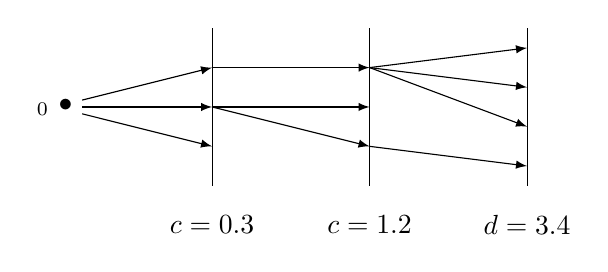
\begin{tikzpicture}
            \node (v0) at (-1,0) {$\sommet{}_0 ~\bullet$};
            \draw (1,1) -- (1,-1);
            \draw (3,1) -- (3,-1);
            \draw (5,1) -- (5,-1);
            \node (tmp) at (1,-1.5) {$c=0.3$};
            \node (tmp) at (3,-1.5) {$c=1.2$};
            \node (tmp) at (5,-1.5) {$d=3.4$};
            \draw[-latex] (v0) -- (1,0.5);
            \draw[-latex] (v0) -- (1,0);
            \draw[-latex] (v0) -- (1,-0.5);
            \draw[-latex] (1,0.5) -- (3,0.5);
            \draw[-latex] (1,0) -- (3,0);
            \draw[-latex] (1,0) -- (3,-0.5);
            \draw[-latex] (3,0.5) -- (5,0.75);
            \draw[-latex] (3,0.5) -- (5,0.25);
            \draw[-latex] (3,0.5) -- (5,-0.25);
            \draw[-latex] (3,-0.5) -- (5,-0.75);
        \end{tikzpicture}
    \end{center}

    Si tous les coûts sont à 1 ($\forall \arc{}\in \arcs{}, \cout{}(\arc{})$) on retrouve le parcours en largeur.
}

\frame{
    \frametitle{Un tas particulier~: la file de priorité}

    Comme le parcours en largeur ou en profondeur, l'algorithme de Dijkstra s'obtient en utilisant un tas particulier pour faire le parcours générique vu dans les cours précédents.

    \vspace{0.5cm}

    \definition[file de priorité]{%
    Chaque élément du tas possède une priorité associée (un nombre qui permet de classer les éléments).
        \begin{description}
            \item[observer] obtenir l'élément de plus petite priorité
            \item[extraire] retirer l'élément de plus petite priorité
        \end{description}
    }
}

\frame{
    \frametitle{Algorithme de Dijkstra}

    \begin{center}
        \begin{minipage}{10cm}
            \begin{algorithmic}
                \In{$\grapheval{}$, $\sommet{}_0\in\sommets{}$}
                \Out{$g$, $pred$}
                \State $g(\sommet{}_0) = 0$
                \State $t = init()$ \enavant{// file de priorité où on utilise $g$ comme priorité}
                \State $t.ajouter(\sommet{}_0)$
                \State marquer $\sommet{}_0$
                \While{$!t.estVide()$}
                    \State $\sommet{} = t.observer()$
                    \State $t.extraire()$
                    \ForAll{$\sommetb{}, (\sommet{}, \sommetb{})\in\arcs{}$}
                        \If{$g(\sommetb{}) > g(\sommet{}) + \cout{}((\sommet{}, \sommetb{}))$}
                            \State $g(\sommetb{}) = g(\sommet{}) + \cout{}((\sommet{}, \sommetb{}))$
                            \State $pred(\sommetb{}) = \sommet{}$
                            \If{$\sommetb{}$ non marqué}
                                \State marquer $\sommetb{}$
                                \State $t.ajouter(\sommetb{})$                            
                            \EndIf
                        \EndIf
                    \EndFor
                \EndWhile
            \end{algorithmic}
        \end{minipage}
    \end{center}
}

\frame{
    \frametitle{Exemple}

    \exercice{%
        Appliquer l'alogrithme de Dijkstra au graphe suivant pour $\sommet{}_0 = \sommet{}_1$.
        \begin{center}
            \begin{tikzpicture}
                \node (v3) at (0,0) {$\sommet{}_3$};
                \node (v4) at (3,0) {$\sommet{}_4$};
                \node (v1) at (0,3) {$\sommet{}_1$};
                \node (v2) at (3,3) {$\sommet{}_2$};
                \node (v5) at (6,0) {$\sommet{}_5$};

                \shiftdraw{v1}{v2}{0}{0};
                \shiftdraw{v1}{v4}{0}{0};
                \shiftdraw{v2}{v4}{0}{0};
                \shiftdraw{v3}{v1}{0}{0};
                \shiftdraw{v4}{v3}{0}{0};
                \shiftdraw{v5}{v4}{0}{0}; 

                \node (info) at (1.5, 3.2) {2};
                \node (info) at (1.5, -0.2) {2};
                \node (info) at (-0.2, 1.5) {2};
                \node (info) at (3.2, 1.5) {2};
                \node (info) at (4.5, -0.2) {0};
                \node (info) at (1.7, 1.7) {-1};
            \end{tikzpicture}
        \end{center}
    }
}

\frame{
    \frametitle{Preuve de l'algorithme}

    \proposition{%
        Pour tout graphe $\graphe{}$, l'algorithme de Dijkstra termine.
    }

    \exercice{%
        Prouver cette proposition.
    }

    \pause

    \proposition{%
        À la fin de l'exécution de l'algorithme de Dijkstra sur un graphe $\graphe{}$, $pred(\sommet{})$ est défini si et seulement si il y a un chemin de $\sommet{}_0$ à $\sommet{}$ dans $\graphe{}$.
    }

    \exercice{%
        Prouver cette proposition.
    }
}

\frame{
    \frametitle{Preuve de l'algorithme, suite}

    \proposition{%
        À n'importe quel moment de l'exécution de l'algorithem de Dijkstra sur un graphe $\graphe{}$, si $\sommet{}$ est marqué mais n'est pas dans la file, alors $g(\sommet{})$ (et donc $pred(\sommet{})$) ne change plus jamais.
    }

    \exercice{%
        Prouver cette proposition.
        On peut le faire par l'absurde en supposant qu'il existe un sommet $\sommet{}$ qui est marqué, en dehors de la file et pour lequel $g(\sommet{})$ change.
    }
}

\frame{
    \frametitle{Preuve de l'algorithme, fin}

    \proposition{%
        Lorsqu'on exécute l'algorithme de Dijkstra sur un graphe $\graphe{}$, au moment où un sommet $\sommet{}$ sort de la file $pred(\sommet{})$ permet de retrouver un chemin de coût minimum de $\sommet{}_0$ à $\sommet{}$ et $g(\sommet{})$ est le coût de ce chemin.
    }

    \remarque{%
        Le chemin en question est $pred^n(\sommet{})pred^{n-1}(\sommet{})\dots pred(\sommet{})\sommet{}$ avec $pred^n(\sommet{}) = \sommet{}_0$.
    }

    \pause

    \exercice{%
        Prouver cette proposition.
        On pourra commencer par prouver que $pred$ définit bien des chemins avant de montrer que ces chemins sont de coût minimum.
    }
}